%!TEX root = /Users/simo/Documents/PFC/Chapter3/chapter3.tex
\section{Tercer Ciclo} % (fold)
\label{sec:tercer_ciclo}

En estos momentos un usuario puede crear y editar sus documentos, pero aún no existe ningún tipo de seguridad a la hora de trabajar desde la pizarra. Puesto que la idea original para esta aplicación, es que los usuarios podrían acceder a documentos dependiendo de los permisos que se le hubiera dado, tanto por la parte del grupo como independientemente. Para este ciclo, el objetivo será la introducción del concepto Grupo, de forma que se puedan agrupar usuarios de forma sencilla y rápida, y que se puedan asignar en un futuro, permisos de forma rápida a estos grupos de gente.

\subsection{Análisis de requisitos} % (fold)
\label{sub:análisis_de_requisitos}

\begin{itemize}
  \item Poder crear, editar y borrar grupos.
  \item Un grupo deberá tener un dueño, que será el creador, que siempre tendrá los máximos permisos, y que podrá invitar, echar y promocionar a otros usuarios. Una vez invitado, un miembro puede ser promocionado a administrador, de forma que pueda a su vez, invitar, promocionar y echar a gente. Un administrador no puede eliminar el grupo o echar / degradar a otros administradores, privilegios reservados al dueño del grupo.
  \item Los usuarios invitados pueden aceptar o rechazar las invitaciones, además de sarlir del grupo voluntariamente, después de ser invitado. Para evitar una avalancha de invitaciones, solo un usuario puede invitar a un usuario a un grupo.
\end{itemize}

% subsection análisis_de_requisitos (end)

\subsection{Diseño} % (fold)
\label{sub:diseño}

\begin{figure}[h!]
\centering
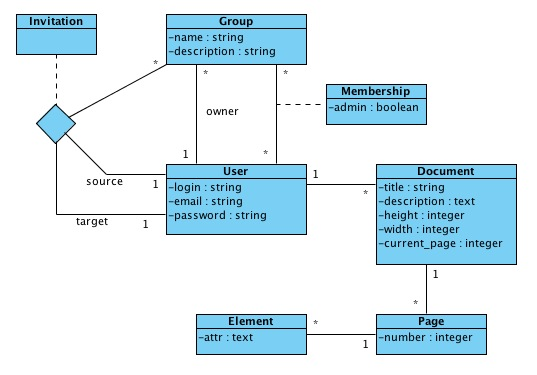
\includegraphics[width=14cm]{uml3.png}
\caption{Clases del dominio, 3er ciclo}\label{fig:uml3}
\end{figure}

En este paso se hace todo el sistema de clases un tanto más complejo. Un grupo tiene una relación doble con la clase \texttt{User}, teniendo un dueño, y múltiples usuarios. Además, puesto que los miembros pueden ser administradores, existen dos posibilidades. Una sería tener una triple relación, de dueño, administradores y usuarios normales; la otra sería tener una clase asociativa \texttt{Membership}, que contenga la información de si este miembro tiene permisos de administrador o no. La segunda opción se cree más eficiente, puesto que siempre será más fácil modificar un atributo de la tabla \texttt{Membership} que destruir una relación y crear otra nueva, además de simplificar el proceso de encontrar todos los miembros de un grupo, sean administradores o no.

En cuanto al proceso de realizar invitaciones, es necesario almacenar de alguna forma temporal dichas invitaciones, y la solución natural es una asociación terniaria entre un grupo y dos usuarios, el que invita (source) y el invitado (target).

Por desgracia Ruby on Rails aún no soporta relaciones asociativas, debiéndose por tanto normalizar el diagrama antes de poder traducirse a la estructura de modelos.

\begin{figure}[h!]
\centering
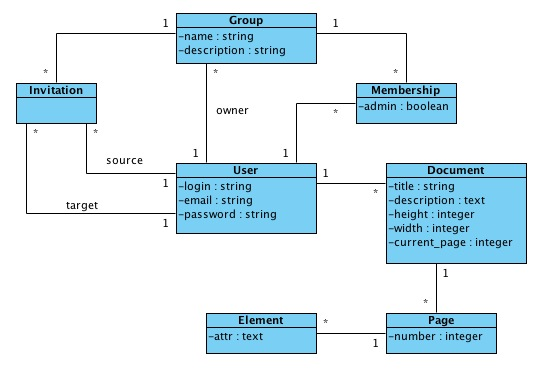
\includegraphics[width=14cm]{uml3n.png}
\caption{Clases del dominio, 3er ciclo, diagrama normalizado}\label{fig:uml3n}
\end{figure}

En cuanto a modelos, se cree necesario crear un nuevo controlador para todas las acciones referentes a los grupos

% subsection diseño (end)

\subsection{Implementación} % (fold)
\label{sub:implementación}

A pesar de la nueva complejidad de las clases introducidas (tres nuevas clases, con un total de seis nuevas relaciones), el proceso de traducción de este diagrama a clases es púramente burocrático. El peso de controlar las restricciones dejadas atrás por la normalización recae sobre los controladores, que a la hora de invitar a gente se deberá comprobar que no sea miembro y que no haya sido invitado ya.

% subsection implementación (end)

% section secundo_ciclo (end)